
\subsection{Estimate Anomaly Detection Quality 
without Test Label}

In this section, we evaluate Algorithm 
\ref{alg:anomalydetection} 
with four representative anomaly detection models, 
including one-class SVM, PCA, k-means and GMM. 
Again, we first present a case study and then other results. 

\begin{table*}[t]
\centering
\renewcommand{\arraystretch}{1.5}
\caption{Conditional Predictive Demographic Disparity on the 
Crime Community Data Set}
% \centering
\begin{tabular}{l|ccccc|ccccc} \hline 
\bf Classifier & \bf $\gamma_{+}(f; Q)$ & \bf $\gamma_{+}(f; S)$ 
& \bf $\gamma_{+}(f_{q}; S)$ & \bf $\Delta_{tr}$ & 
\bf $\Delta_{retr}$ & \bf $\gamma_{-}(f; Q)$ & \bf $\gamma_{-}(f; S)$ 
& \bf $\gamma_{-}(f_{q}; S)$ & \bf $\Delta_{tr}$ & 
\bf $\Delta_{retr}$ \\ \hline 
LogitRegressor & .316 (4e-3) & .368 (3e-3) & .246 (3e-3) & .052 & .070 
& .034 (2e-4) & .030 (1e-4) & .027 (7e-5) & .004 & .008 \\ 
LSVM & .300 (3e-3) & .376 (4e-3) & .297 (4e-3) & .076 & .003 
& .039 (2e-4) & .024 (2e-4) & .024 (1e-4) & .015 & .014\\ 
k-NN & .290 (4e-3) & .419 (6e-3) & .262 (6e-3) & .129 & .029 
& .056 (4e-4) & .044 (3e-4) & .026 (3e-4) & .012 & .030\\  
DecisionTree & .364 (2e-2) & .451 (2e-3) & .384 (2e-2) & .087 & .020 
& .072 (1e-3) & .060 (2e-3) & .067 (3e-3) & .012 & .004\\  \hline 
\end{tabular}
\label{exp1:disparity}
\end{table*}

{\noindent \bf A Case Study on Spam Email Data Set} 

We formalized an anomaly detection task by considering 
spam emails as anomalies. Recall that only normal 
instances were used to train model at first, but all 
training instances were used to evaluate the retrained model.
One-class linear SVM was used as the base detection model. 
Its regularization coefficient was set to 1e-3 based on 
results in Figure \ref{exp1:anomalymodelselection}. 

\begin{figure}[h]
\centering
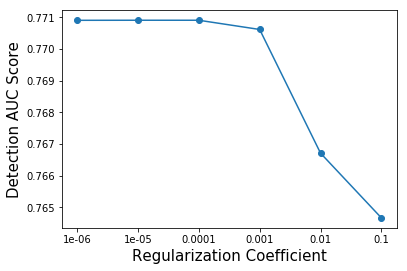
\includegraphics[width=4.5cm,height=3.25cm]{exp1_anomalymodelselection.png}
\vspace{-10pt}
\caption{Testing Error versus Regularization Coefficient}
\label{exp1:anomalymodelselection}
\end{figure}

We evaluated AUC score. Recall $AUC(f; Q)$ is the 
testing score and $AUC(f; S)$ is the training score. 
Let $\widetilde{AUC}(f; S)$ be the reversed testing score. 
The estimation quality of $AUC(f; S)$ on $AUC(f; Q)$ is 
\begin{equation}
\Delta_{tr} = | AUC(f; Q) - AUC(f; S) |,  
\end{equation}
and the estimation equality of $\widetilde{AUC}(f; S)$ 
on $AUC(f; S)$ is 
\begin{equation}
\Delta_{retr} = | AUC(f; Q) - \widetilde{AUC}(f; S) |.  
\end{equation}

Results in Table \ref{exp1:anomalyaucscore} show 
reversed AUC score is a more accurate 
estimate of testing AUC score than training AUC. 

\begin{table}[h]
\renewcommand{\arraystretch}{1.5} 
\caption{Anomaly Detection AUC Scores on Spam Email Data Set}
\centering
\begin{tabular}{ccccc} \hline 
$AUC(f; Q)$ & $AUC(f; S)$ & $AUC(f_{q}; S)$ 
& $\Delta_{tr}$ & $\Delta_{retr}$ \\ \hline 
.7709 & .7733 & .7705 & .0024 & .0004 \\ \hline 
\end{tabular}
\label{exp1:anomalyaucscore}
\end{table}

Next, we evaluated the impact of sample size on 
estimation quality and obtained results in 
Figure \ref{exp1:anomalysamplesize}. 
We see reversed AUC score is more effective when 
training sample and testing sample are more balanced. 
This is different from our observations in 
classification tasks. 

\begin{figure}[h]
\centering
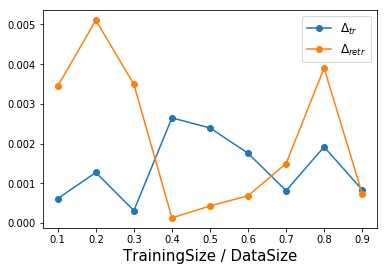
\includegraphics[width=5.5cm,height=3.5cm]{exp1_anomalysamplesize.png}
\vspace{-10pt}
\caption{$\Delta_{tr}$ and $\Delta_{retr}$ versus Training 
Sample Size} 
\label{exp1:anomalysamplesize}
\end{figure}

Finally, we evaluated the impact of label confidence 
on estimation quality. We used $70\%$ data for training 
and the rest for testing. 
We used only confidently pseudo-labeled normal instances 
to retrain $f$, 
and obtained results in Figure \ref{exp1:anomalyconfidence}. 
We see reversed AUC score becomes a better estimate 
as one uses fewer confidently pseudo-labeled instances 
for retraining, but it remains less accurate than 
training AUC score.  

\begin{figure}[h]
\centering
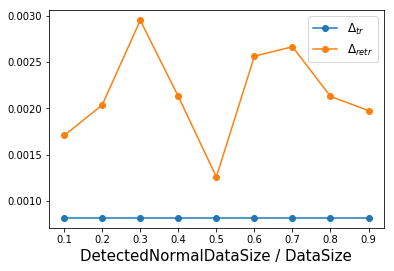
\includegraphics[width=5.5cm,height=3.5cm]{exp1_anomalyconfidence.png}
\vspace{-10pt} 
\caption{$\Delta_{tr}$ and $\Delta_{retr}$ versus Different 
Fractions of Identified Normal Instances. (TraininSize/DataSize=0.7)}
\label{exp1:anomalyconfidence}
\end{figure}

{\noindent \bf Results on other Data Sets with 
other Models} 

Now we evaluate Algorithm \ref{alg:anomalydetection} 
extensively on several data sets based on 
multiple detection models. 
Results are shown in Table \ref{tab1:auc}. 
We see $\widetilde{AUC}(f; S)$ is consistently 
a more accurate estimate of $AUC(f; Q)$ than 
$AUC(f; S)$. 

% \begin{table*}[t!]
% \renewcommand{\arraystretch}{1.5} 
% \caption{Z-Scores of all the data sets used in the experiments}
% \centering
% \begin{tabular}{|l|c|c|c|c|c|c|c|c|} \hline 
% \bf Data Set & Spam Email & Satellite & Cardio & Ionosphere & Malware & Network Intrusion & Arrhythmia \\ \hline 
% \bf Z-Score & 2e-4 & 2e-3 & 5e-4 & 1e-2 & 2e-5 & 4e-5 & 3e-4 \\  \hline 
% \end{tabular}
% \label{exp1:disparity}
% \end{table*}
